%\renewcommand{\contentsname}{CONTENTS}
%\renewcommand{\bibname}{Bibliography}
%\renewcommand{\indexname}{INDEX}
%\renewcommand{\figurename}{図 }
%\renewcommand{\tablename}{表 }
%\renewcommand{\appendixname}{APPENDIX}

\renewcommand{\part}{Contents}
\renewcommand{\prechaptername}{第 }
\renewcommand{\postchaptername}{ 章}

\chapter{序論}
 
本章では、最初に本研究における背景およびその現状の問題点を述べる。
そのあと、これに対する本研究の目的とアプローチについて述べる。
そして最後に、本論文の構成について示す。

\section{背景}
私たちの身の回りには様々なIoT製品が存在している。
そのうち、最も身近な例はスマートフォンであろう。 \\
Google Now\cite{google_now}は生活の中において、必要な情報を聞く前に教えてくれる技術である。
下図\ref{GoogleNow}\footnote{\url{https://www.google.com/intl/ja/landing/now} (2018年1月23日確認) より引用}にそのスクリーンイメージを示した。
例えば、夜遅くまで外にいるとき、ユーザがスマホに聞くことなく終電の時間を教えてくれる機能がある。
これはスマートフォンのGPS機能と、現在時刻、交通機関のダイヤを参照した上でユーザに通知を与えているものである。 \\
\begin{figure}[htbp]
 \centering
  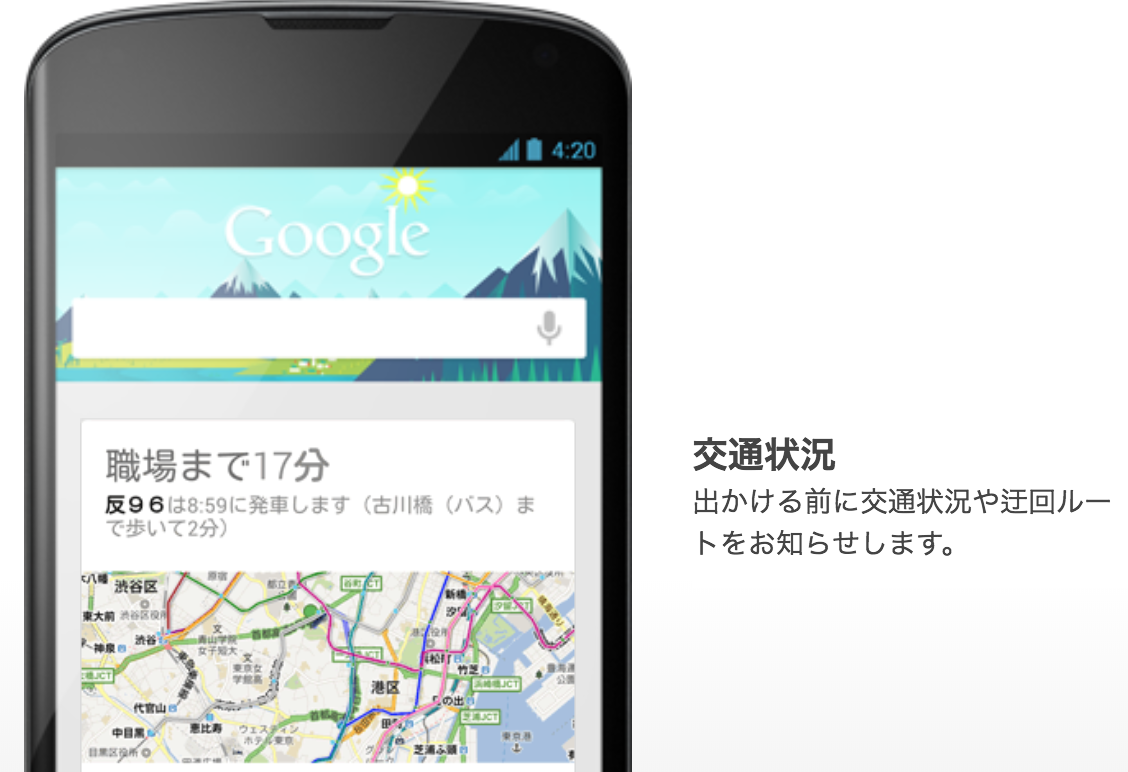
\includegraphics[width=70mm]{image/GoogleNow.png}
 \caption{Google Nowのスクリーンイメージ}
 \label{GoogleNow}
\end{figure}
他にも、ウェアラブルデバイスが注目されている。
fitbit\cite{fitbit}は腕時計式のウェアラブルデバイスである。
アプリをインストールすると、デバイスから取得した歩行数や心拍数、睡眠時間、食事、消費カロリーなどのデータを閲覧できる。
下図\ref{fitbitImage}\footnote{\url{https://www.fitbit.com/jp/purepulse} (2018年1月23日確認) より引用}にそのスクリーンイメージを示した。
\begin{figure}[htbp]
 \centering
  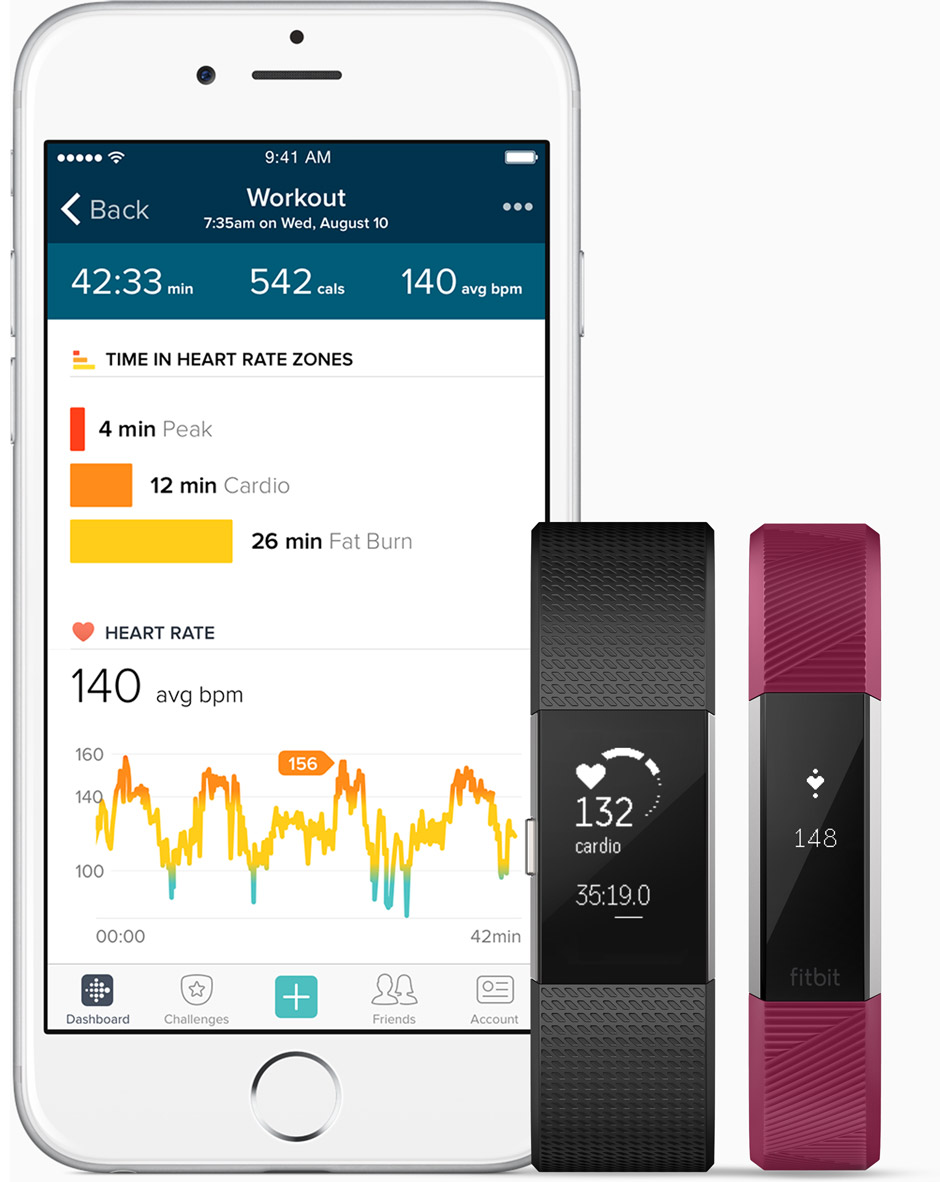
\includegraphics[width=70mm]{image/fitbit.png}
 \caption{fitbitのスクリーンイメージ}
 \label{fitbitImage}
\end{figure}
これをもとに運動や食事の計画を立てることができ、健康維持に役立てることができる。 \\
他にも、車にカメラを取り付けることで道路上の白線の掠れを検知し、塗り直すべき白線の箇所を取得する研究\cite{dragnman_hakusen}がある。
これによって、今までは別途調査が必要であった道路の白線の掠れている場所の検知が簡単になり、自治体が行っている白線の掠れの調査に関するコストを削減できることが期待されている。 \\
このように、IoT製品\UTF{00B7}サービスは様々な利益を我々に与えてくれている。
そしてこれらのIoT製品\UTF{00B7}サービスは全て取得したIoTデータが源となり、我々に有益な状態をもたらしてくれている。
この元のデータなしにIoTの製品\UTF{00B7}サービスは決して生まれない。 \\
そこで、このIoTデータの流動性を高めるため、IoTデータ市場というものが近年、考えられている。
その市場ではIoTデータを事業者間で売買できるようになっていて、取引の際の手数料をこの市場を管理する管理者へ払うようになっている。
他の課金制度としては、この市場に参加する際や、参加し続ける際に管理者へ払うようになっている制度も存在する。
このように一定の仲介手数料は存在するものの、IoTデータをより簡単に調達できるようになるIoTデータ市場は、買い手にとって利益をもたらしてくれるものである。
またこのIoTデータ市場は売り手にとっても、今まで自社でしか活用用途のなかったデータを販売することが可能になる点で、利益を得られる。
このように、IoTデータ市場は買い手と売り手の双方にとって利益を享受することのできるものであるため、これからIoT市場全体の成長に伴って出現\UTF{00B7}発展していくものと考えられている。 \\
このIoTデータ市場が日本において最大の規模で実現されているのがEverySense\cite{everysense}である。
下図\ref{everysense}\footnote{\url{https://every-sense.com} (2018年1月23日確認) より引用}にその取引のイメージをまとめた画像を示す。
\begin{figure}[htbp]
 \centering
  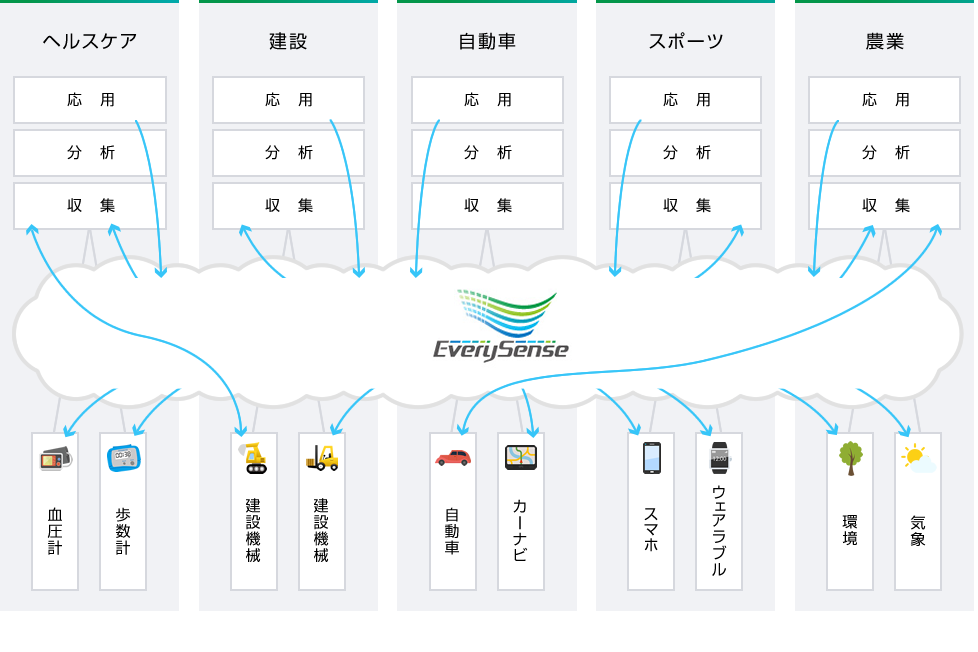
\includegraphics[width=120mm]{image/everysense.png}
 \caption{EverySenseにおけるIoTデータ市場イメージ}
 \label{everysense}
\end{figure}
このように、IoTデータ市場は業界の垣根を超えて様々なデータを簡単に取得することが可能となるプラットフォームである。

\section{IoTデータ市場に関する問題}
IoTデータ市場は寡占状態になりやすい市場である。
現在、日本におけるeコマース市場のプラットフォームで大きなシェアを占めているものと言えば、Alibabaやamazonである。
これに対抗しようと、これから新規でeコマース市場を立ち上げたとしても、これらに勝る何かの機能がないと難しいだろう。
多くの販売者と購買者という参加者が存在する既存の市場から、参加者の少ない市場へとユーザが誘導されるための動機付けがないためだ。
しかし実際の店舗で考えると、既存の店舗と全く同じ店舗を1km離れたところに作ったとすると、そちらの方が近くて便利と感じるユーザが新規店舗へと流れる。
このように実世界と違い、ネットワークにおいては先行者利益がとても大きいものであるのだ。
そして、IoTデータ市場は実社会に店舗を構えるスタイルの市場ではない。
よって先行者利益によって、いくつかの市場の管理者が大きな力を持ち、IoTデータ市場全体を支配することが可能である。
amazonはeコマースの世界では多くのシェアを占めているが、これらで買える商品は実在する実店舗でも購入できることが多い。
したがって、eコマースという形態の市場において影響力を持つが、このプラットフォーム上で売買される商品に関する市場全体をコントロールする力を持つわけではない。
しかし、IoTデータ市場は実社会の店舗を持たないため、この市場の管理者がIoTデータという商品自体に関する市場全体を支配することになるのだ。
詳しくは2.2節にて後述するが、これは公正な取引が行われにくくなるというリスクを孕む。
よって、IoTデータ市場には管理者がいない方が望ましい。
しかし、現状は管理者の存在するIoTデータ市場しか存在しない。
本研究ではこれが問題であると考える。

\section{目的とアプローチ}
本研究の先にある最終の目的は、利用者にとって自由の割合と支配の割合が各々の利用者にとって最も理想的な塩梅で行われているIoTデータ市場を構築することである。
具体的に述べると、最終目的にある市場は利用者の意思や希望と関係なく、技術的に仕方なく存在していたIoTデータ市場の巨大な管理者という存在を、利用者が選ぶ各々にとって必要な分のルールや管理者よって透明な形で提供するものである。
そこで本研究では現実世界の市場と同じように、一つの組織にも囚われない、オープンなIoTデータ市場を作ることをアプローチとする。
そして本研究の先に、利用者にとって必要なルールや必要とされる管理団体が存在するIoTデータ市場が構築される取り組みが存在するべきである。
この手法を取る理由は、今までの中央集権的なシステムを発展させてより管理団体の権限を減らすことは技術的に難しいが、本研究で提示する手法を発展させて管理者やルールを作ることは可能であるためである。
これらの考えを図にして表すと下図\ref{distributed}\footnote{\url{https://medium.com/distributed-economy/what-is-the-difference-between-decentralized-and-distributed-systems-f4190a5c6462} (2018年1月23日確認)より引用、一部改変} のようになる。
\begin{figure}[htbp]
 \centering
  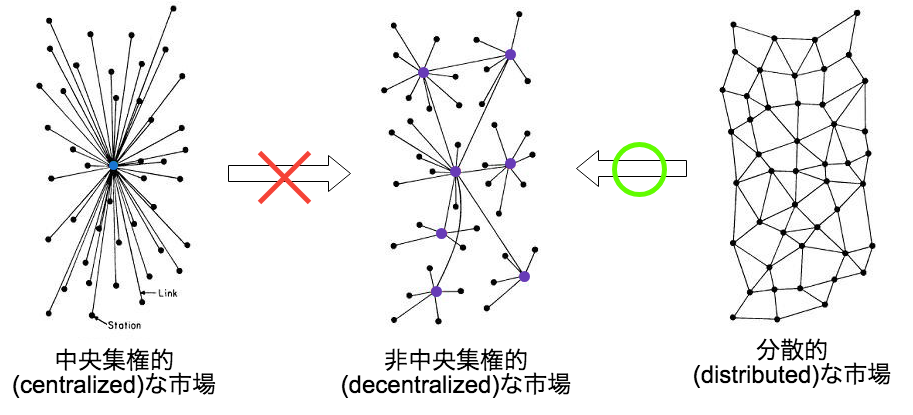
\includegraphics[width=140mm]{image/CentralizedDistributed.png}
 \caption{centralized, decentralized, distributedに関する図}
 \label{distributed}
\end{figure}
そして本研究のように中央集権を無くす際、管理者のいない中での合意アルゴリズムが必要となるが、これにはブロックチェーンを使用する。
また、データの買い手と売り手の間でのデータ通信が必要となるが、これにはメッセージングシステムを使用する。
この二つを統合させ、IoTデータ市場を作り出すことが本研究の技術的なアプローチである。

\section{本論文の構成}
本論文は本章を含めて8章からなる。
本章ではIoTが我々の生活の役に立っていることと、そのためにはデータが不可欠でその市場が誕生していること、しかしそこには管理者がいるという問題点が存在することを示した。
また、それに対する目的とアプローチを述べた。
2章ではこれをさらに詳細に、技術的な観点も含めて論じる。
3章ではブロックチェーン技術について簡単に述べ、今回使用するEthereumやオフチェーン技術について触れる。
4章では提案するIoTデータ市場の機能要件およびそのプラットフォーム上での取引の流れを述べる。
5章では提案する市場に関して、設計と実装を述べる。
6章では提案する市場に関して、トランザクション流通量などの定量評価を行う。
7章では今後の展望について、ブロックチェーン技術の観点と社会的な観点から論じる。
8章では本論文のまとめを述べる。